\documentclass[10pt,a4paper]{article}
\usepackage[utf8]{inputenc}
\usepackage[dutch]{babel}
\usepackage{amsmath}
\usepackage{amsfonts}
\usepackage{amssymb}
\usepackage{graphicx}
\usepackage{color}
 
\definecolor{codegreen}{rgb}{0,0.6,0}
\definecolor{codegray}{rgb}{0.5,0.5,0.5}
\definecolor{codepurple}{rgb}{0.58,0,0.82}
\definecolor{backcolour}{rgb}{0.95,0.95,0.92}
\usepackage{listings}
\lstdefinestyle{cstyle}{
    backgroundcolor=\color{backcolour},   
    commentstyle=\color{codegreen},
    keywordstyle=\color{magenta},
    numberstyle=\tiny\color{codegray},
    stringstyle=\color{codepurple},
    basicstyle=\footnotesize,
    breakatwhitespace=false,         
    breaklines=true,                 
    captionpos=b,                    
    keepspaces=true,                 
    numbers=left,                    
    numbersep=5pt,                  
    showspaces=false,                
    showstringspaces=false,
    showtabs=false,                  
    tabsize=2
}
\graphicspath{ {./images/} }

\begin{document}
\begin{titlepage}
    \centering
    \vfill
    {\Large
        Robotica: Hexapod\\
        \vskip2cm
        I. van Alphen, S. van Doesburg, E.  Salsbach, M. Visser\\
    }    
    \vfill
    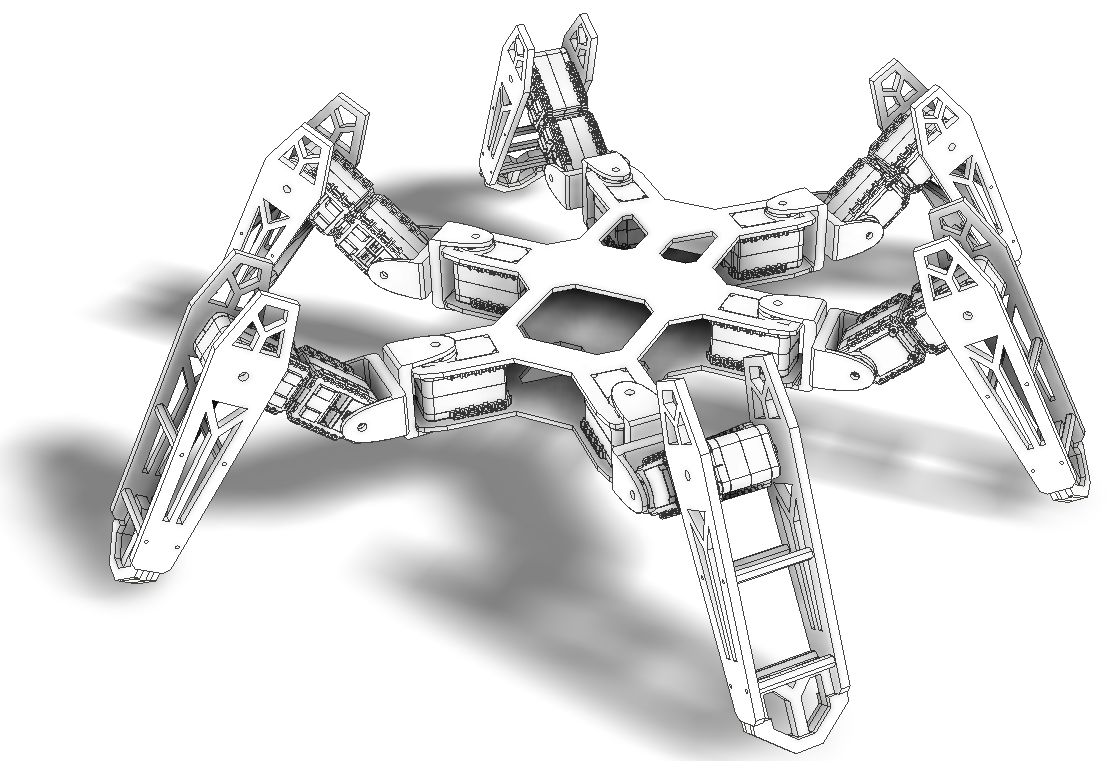
\includegraphics[width=1\textwidth]{WireS4}
    \vfill
    \vfill
\end{titlepage}

\newpage

\tableofcontents
\newpage

\iffalse % Commentaar sectie
\section{Samenvatting}
Not in use yet
\newpage
\fi



\section{Inleiding}
Deze opdracht betreft het ontwikkelen van de besturing en simulatie van een hexapod robot.\cite{beroepsopdrachten} De robot die gebruikt gaat worden is de PhantomX AX Hexapod van TrossenRobotics. \cite{PhantomX AX Hexapod Kit}.

In de huidige situatie wordt een hexapod handmatig met een afstandbediening bestuurd en kent geen vorm van intelligentie. Ter voorbereiding op het werken met kunstmatige intelligentie, is er voor gekozen om een simulatiemodel van de robot te ontwikkelen. Om praktische informatie te verzamelen is er een koppeling nodig tussen het simulatie model en de hardware van de robot. Met behulp van deze koppeling kan er onderzoek gedaan worden naar bijvoorbeeld effici\"ente looppatronen en zelf lerende functies.

Het verslag is opgebouwd uit het onderzoek naar een hexapod met daarbij de hoofdvraag en deelvragen. Gevolgd door de specificaties en de implementatie van het ontwerp.

\newpage

\section{Opdrachtdefinitie} 
De hexapod is momenteel alleen te besturen met behulp van een afstandbediening. De huidige besturingssoftware op de robot is niet in staat naast de afstandbediening om externe commando's te verwerken. Daarnaast kent het in de huidige toestand geen vorm van intelligentie. Zo heeft de robot momenteel geen besef van wat zich in zijn directe omgeving bevindt.

Als voorbereiding op het werken met kunstmatige intelligentie op de robot, is er voor gekozen om een simulatiemodel voor en van de robot te ontwikkelen. De redenen hiervoor zijn onder andere dat er in een model oneindig veel verschillende situaties voor de robot gecree\"erd kunnen worden. Hiernaast is het simuleren van de hexapod sneller dan real-time testen en is er minder kans op schade van het materieel. Bovendien kan het vanuit financie\"el oogpunt in situaties nuttig zijn om niet met de echte hardware van de robot te werken. 
Door een real-time koppeling te maken tussen het simulatiemodel en de hardware van de robot is het mogelijk in staat om meer informatie te verzamelen om de intelligentie te verbeteren.

Het uiteindelijke doel is om in een simulatieomgeving de bewegingseigenschappen van de robot te optimaliseren om deze software vervolgens te testen op het echte model. Er moet dus onderzocht worden hoe een ontwikkelingsomgeving opgezet kan worden waarbij er een koppeling is tussen een simulatie en de robot zelf. Daarnaast moet de robot extern te besturen zijn met behulp van een computer. De robot en het simulatiemodel moeten de mogelijkheid hebben om de stand van de servomotoren real-time naar elkaar over te brengen. Om beschadiging te voorkomen moet het in staat kunnen zijn om fouten te detecteren. De onderlinge poten zouden niet met elkaar in contact moeten komen. Het onderzoeken van het gedrag van een hexapod is van belang om uiteindelijk de hexapod zelf lerende functies te geven.
\newpage

\iffalse %commentaar sectie
\textbf{Hoofdvraag\\}
De hoofdvraag van het onderzoek betreft:
Hoe wordt een ontwikkelingsomgeving opgezet waarbij een robot aan een simulatie gekoppeld wordt?

\textbf{Deelvragen\\}
De onderzoeksvraag is onder te verdelen in verschillende deelvragen:
\begin{itemize}
\setlength\itemsep{0em}
\item Wat is een hexapod?
\item Welke draadloze techniek kan het beste worden toegepast als communicatiemiddel?
\item Wat zijn effici\"ente looppatronen voor een hexapod op verschillende oppervlakken?
\item Is een hexapod in staat om zich voort te bewegen met één of meerdere beperkingen aan zijn poten?
\item Zijn er effici\"entere looppatronen bij een zwaardere belasting van de hexapod?
\item Zijn er verschillen tussen de simulatie en de werkelijkheid?
\item Hoe detecteert de hexapod dat er een onmogelijke bewegingsactie uitgevoerd moet worden?
\item Hoe verkent de hexapod zijn omgeving en onderscheid deze objecten van elkaar?
\item Kan de robot zich voortbewegen ongeacht de orie\"entatie?
\end{itemize}
\fi

\section{Onderzoeks opzet}
Het project bestaat uit twee delen. Het eerste deel heeft als doel de hexapod in de simulatie te verwerken. Het tweede deel is ervoor zorgen dat er een verbinding ontstaat tussen de simulatie en de hexapod. 
Vanwege de wensen van de opdrachtgever zal er gewerkt worden met het simulatie-programma V-REP en zullen andere softwarepakketten buiten beschouwing worden gelaten.  

Daarnaast zal er in de eerste deel gekeken worden naar toepassingen die andere hebben bedacht voor de hexapod. Hieruit is inspiratie te halen voor handige en leuke toepassingen.

Om de verbinding te maken tussen robot en computer dienen er verschillende bronnen te worden geraadpleegd. Een groot deel van die bronnen zal worden voorzien door gebruik te maken van het internet. Verder zal kennis die in de les wordt opgedaan, worden toegepast en de boeken kunnen worden bekeken.


De hexapod is al fysiek aanwezig, wat het testen van geschreven code gemakkelijk maakt. Op deze manier wordt gelijk duidelijk of het geschreven programma functioneert. Tijdens het schrijven van de verschillende functies zal de hexapod fysiek aanwezig zijn om direct het resultaat te ondervinden.

\section{Specificaties}

Voor de specificaties van dit project, is het van belang een onderscheid te maken tussen functionaliteiten die noodzakelijk of gewenst zijn bij het ontwerp. De noodzakelijke functies moeten in ieder geval ge\"implementeerd worden, terwijl het overige optioneel is, afhankelijk van de tijdrestrictie.

\subsection{Noodzakeljke specificaties}
Het primair doel van dit project is om een verbinding te cre\"eren tussen een fysieke robot hexapod en een simulatiemodel. De verbinding tussen hexapod en de computer dient draadloos te zijn ten gunste van de bewegingsvrijheid van de robot. De datasnelheid van moet ook vastgesteld worden om de hexapod zo responsief mogelijk te maken. De hexapod moet aangestuurd kunnen worden door het simulatiemodel in het programma VREP. Veranderingen aan de stand van de poten moeten direct terug te zien zijn in het simulatiemodel. Het model moet in ieder geval bestaan uit een body en 6 ledematen. Ieder ledemaat moet onderverdeeld worden in drie hoofdcomponenten die gescheiden zijn door gewrichten en ook door middel van een gewricht zijn verbonden aan de body. Verder moeten de afmetingen en verhoudingen tot een halve centimeter nauwkeurigheid overeenkomen met de hexapod.
Om te voorkomen dat de hexapod zichzelf kan beschadigen is het noodzakelijk dat de maximale bewegingsvrijheid van de gewrichten (per situatie) wordt uitgerekend of ingesteld. Zodat de poten onderling niet met elkaar botsen of dat de bekabeling beschadigd raakt.

\subsection{Gewenste specificaties}
Er zijn een veel mogelijkheden wat betreft additionele functies die ge\"implementeerd kunnen worden. In deze subsectie zijn een aantal functionaliteiten opgesomd die mogelijk ge\"implementeerd kunnen worden, maar die niet noodzakelijk zijn voor het uiteindelijke eindproduct.

\begin{itemize}
\setlength\itemsep{0em}
\item De hexapod is er zich van bewust als hij ondersteboven is geplaatst, en kan de stand van zijn poten daarop aanpassen. Wanneer de hexapod horizontaal gepositioneerd wordt, dan zorgt dit systeem er voor dat alle poten op of richting de ondergrond zijn geplaatst.
\item Is in staat om zijn poten in- en uit te strekken, zodat het eenvoudig opgeborgen en opgezet kan worden.
\item De spin kan muren en/of objecten detecteren en zijn looproute hier op aanpassen. 
\item Met een beperking aan een of meerdere poten is het in staat om het standaard looppatroon aan te passen.
\item Kan zijn looppatroon aanpassen indien nodig, afhankelijk van het gewicht van de eventuele ballast.
\item Eventuele functionaliteiten zoals aan/uit, stand van poten en bewegingen via de computer kunnen activeren bijvoorbeeld via een console.
\end{itemize}

\subsection{Testplan}
% Of is het echt de bedoeling dat er per specificatie onderdeel uitgelegd wordt hoe die getest en beoordeeld wordt? %
Om te kijken of de specificaties gehaald zijn wordt er als eerst gekeken naar de noodzakelijke specificaties. Deze specificaties zijn zo opgesteld dat deze in ieder geval haalbaar zijn. De haalbaarheid van de gewenste specificaties zijn lastig in te schatten omdat dit veelal buiten onze huidige kennis. Daarom kan het blijken dat een of meerdere specificaties te makkelijk of lastig zijn opgesteld naar mate het onderzoek vordert. In dat geval zal er samen met de begeleider gekeken worden of er een alternatieve specificatie mogelijk is.
Of de resultaten wel of niet voldoen aan de eisen kan in veel gevallen objectief beoordeeld worden door te kijken naar de exacte eisen en de bijbehorende resultaten. Echter is dit bij enkele specificaties niet mogelijk en zal dit met logische redenering en duidelijke uitleg worden ondersteund.
Dit betekent dat de resultaten goed gedocumenteerd worden zodat het bij de conclusie duidelijk is wanneer de specificaties gehaald zijn. Bij twijfel of een specificatie gehaald is zal dit met de begeleider besproken worden.



\newpage

\section{Ontwerp}
Het ontwerp en de hexapod zijn onder te verdelen in verschillende delen: hard- en software. De hardware bestaat uit de hexapod en de hiervoor (zelf) ontwikkelde elektronica. Om de hardware te kunnen gebruiken zijn er ook verschillende programma's geschreven. Om een beeld van te krijgen van de samenhang van het ontwerp met hard- en software zijn er twee blokschema's gemaakt. E\'en schema beperkt zich tot de hexapod en het andere schema tot de externe computer(s). In figuur \ref{fig:blockschematic-spider} en \ref{fig:blockschematic-computer} is deze informatie te vinden.

\begin{figure}[h]
    \centering
    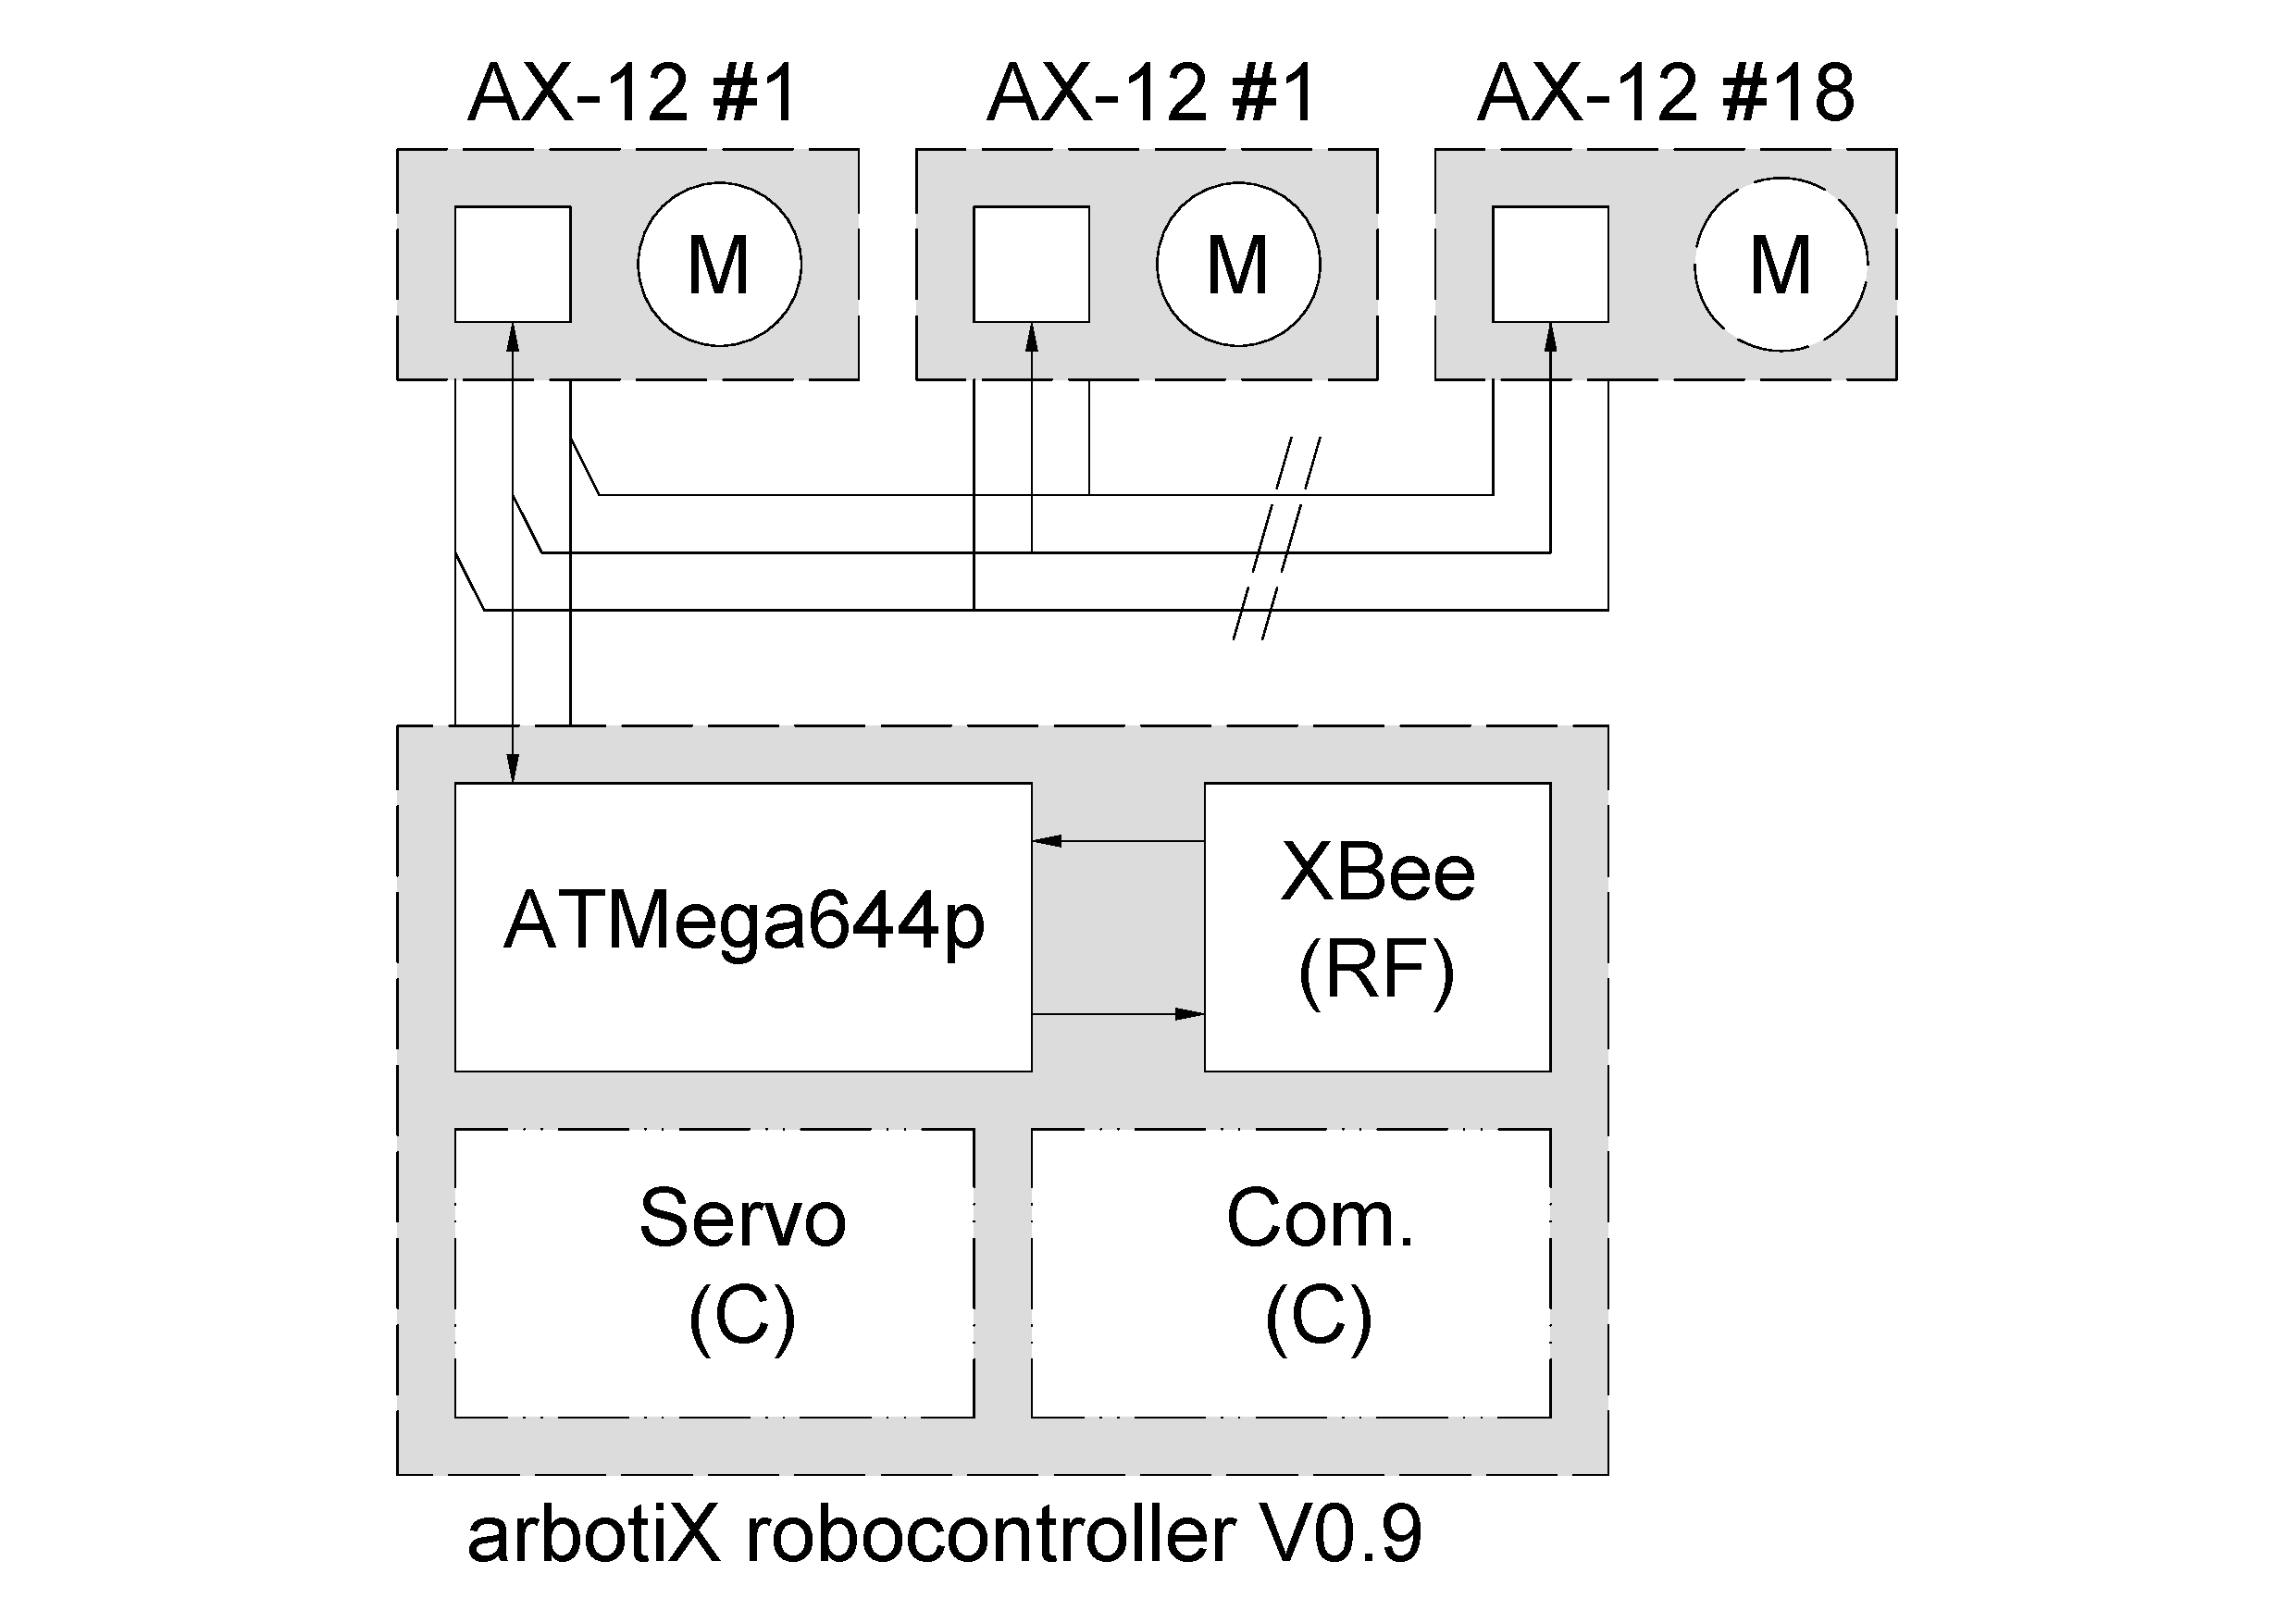
\includegraphics[width=1\textwidth]{blockschematic-spider}
    \caption{Versimpelde weegave in een blokschema van de samenhang van de verschillende systemen en programma's op de hexapod.}
    \label{fig:blockschematic-spider}
\end{figure}

\begin{figure}[h]
    \centering
    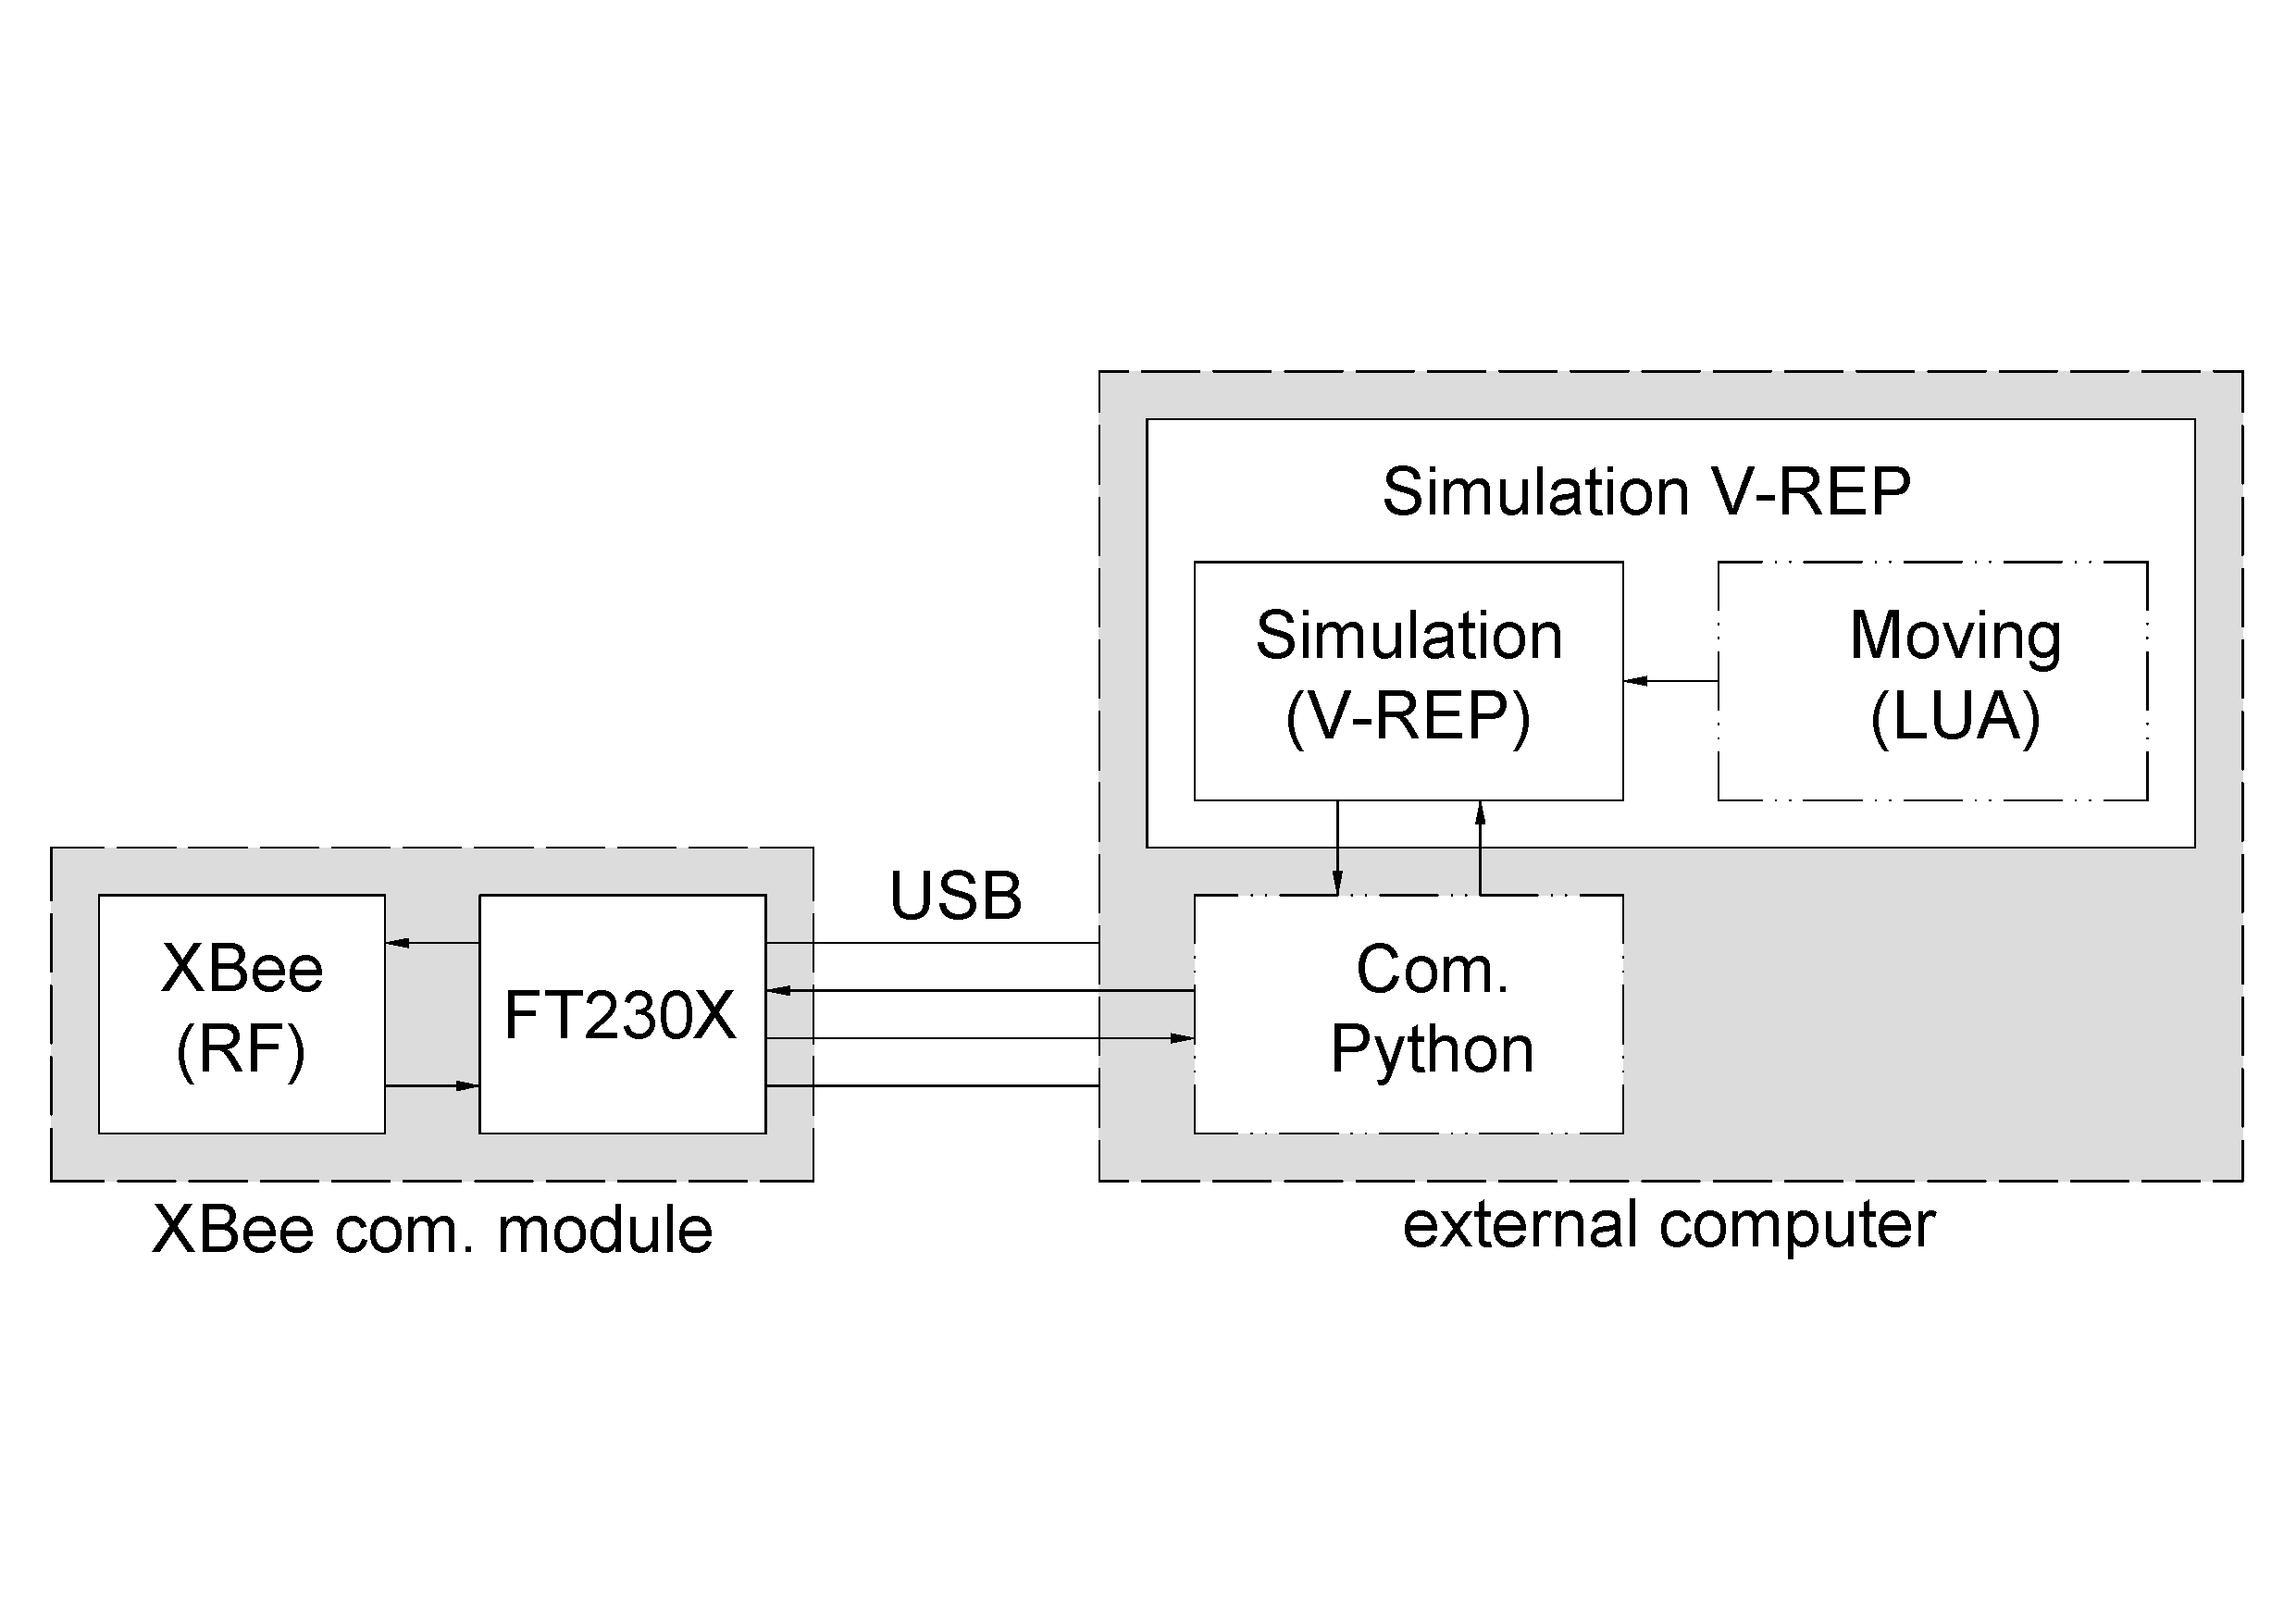
\includegraphics[width=1\textwidth]{blockschematic-computer}
    \caption{Versimpelde weegave in een blokschema van de samenhang van de verschillende systemen en programma's op de externe computer.}
    \label{fig:blockschematic-computer}
\end{figure}

\newpage
\subsection{Het ontwerpen in Inventor}
Het model van de hexapod bestaat uit verschillende componenten. De body bestaat uit twee platen, en elke poot is onder te verdelen in drie onderdelen. Bovendien hoort bij elk gewricht een motor, in totaal 18 motoren. Als eerste zijn de afmetingen van de hexapod zo exact mogelijk opgemeten. Er is maar \'e\'en poot opgemeten, deze is in Inventor vijf maal gedupliceerd. Het programma Inventor geeft de mogelijkheid om met behulp van constraints het voorvlak van elk object te schetsen, en vervolgens uit te breiden tot een driedimensionaal object. Met behulp van constraints, is het mogelijk om alle objecten bij elkaar te voegen.\\

Het driedimensionale model van de robot is gemaakt in het programma Inventor. Dit programma is gekozen omdat dit al bekend is bij de projectleden en gratis te gebruiken voor studenten. Tevens kunnen Inventor bestanden gemakkelijk over worden gezet naar bestanden die leesbaar zijn voor de simulatie software (*.STL).
 
Om de robot te reconstrueren in het tekenprogramma moet de robot gezien worden als losse onderdelen. Elk onderdeel moet apart opgemeten worden met alle hoeken en uitsparingen.

Het model is dan ontleedt tot losse solids (onderdeel bestaande uit een stuk) die samen te voegen zijn tot de uiteindelijke assembly (model opgebouwd uit meerdere onderdelen). De poten bestaan uit drie segmenten die worden verbonden door middel van een servomotor. De poten zijn bevestigd aan de main body. \\



\subsection{De simulatieomgeving}
\subsubsection{Importeren}
Om het inventor bestand te importeren naar V-rep, is het eerst nodig om het model om te zetten naar het STL bestandstype.

Het object wordt initieel in V-rep gezien als geheel object. Met 'divide selected shapes', is het mogelijk om objecten onder te verdelen in zo klein mogelijke stukken. Vervolgens worden die gegroepeerd tot de volgende hoofdonderdelen:

\begin{itemize}
\item Main body + Motor 3(6x)
\item Connector(6x)
\item Motor 1 + 2(6x)
\item Leg(6x)
\end{itemize}

\subsubsection{Gewrichten}
% Dit is zo gekozen om ervoor te zorgen dat er steeds een geheel object gepositioneerd is tussen elk gewricht. % wtf?
 Met behulp van gewrichten worden de 18 pootdelen en de main body met elkaar verbonden. Het is een vrij omslachtig proces om de gewrichten juist toe te voegen. Als allereerst, moet het betreffend hoofdobject geselecteerd worden. Deze wordt vervolgens gekopie\"erd en in een nieuwe scene geplaatst. In 'triangle edit mode', moet het onderdeel geselecteerd worden op de plek waar de joint uiteindelijk hoort te komen. Met 'invert selection', is het mogelijk om het ongewenste deel van het object te selecteren en te verwijderen. In het menu kan er met 'add $\rightarrow$ joint' een gewricht worden toegevoegd. In alle gevallen, wordt er gebruik gemaakt van de 'revolute joint'. Met de functie 'object/item position/orientation' is het mogelijk de joint op exact de zelfde positie als het overgebleven objectonderdeel te plaatsen. Daarbij moet eerst het gewricht geselecteerd worden, en daarna het overgebleven object. In de 'positions/translations' tab moeten de x, y en z co\"ordinaten worden overgenomen. In de 'Orientation/Rotations' map hoort het gewricht zijn juiste ori\"entatie te krijgen. Dit kan door aanpassen van de alpha, beta of gamma waardes. Dit verschilt uiteraard per poot, gezien elke poot een andere ori\"entatie heeft. Als het gewricht eenmaal in de juiste positie is, kan die door middel van kopi\"eren en plakken weer in de originele scene geplaatst worden. De reden dat de 'triangle edit mode' niet gebruikt moet worden in de hoofdscene, is omdat het een grafisch zware operatie is. Bij 'scene object properties' kan overigens de diameter en lengte attributen worden aangepast. Bovendien kunnen de gewrichten daar doorzichtig worden gemaakt.

\subsubsection{Convex en Mask}
% afbeeldingen en illustratie toevoegen! je gebruikt echt heel veel termen die niet altijd duidelijk zijn als je VREP niet kent of geen idee hebt wat VREP uberhaupt is
Omdat V-REP veel berekeningen moet doen bij het simuleren van complexe objecten, is het niet gunstig om te gaan simuleren met de objecten die ge\"importeerd zijn. Het is daarom ook nodig om de vorm van de objecten te vereenvoudigen. Dit kan met 'Morph selection into convex shapes', dat zorgt er uiteindelijk voor dat simulaties vele malen vloeiender worden uitgevoerd. 
Om het uiterlijk van de spin te behouden, worden de ge\"importeerde objecten gebruikt als mask. Om dit te bereiken, moet in het 'dynamic properties dialog' venster alles worden uitgevinkt. Dat zorgt ervoor dat het object niet met zijn omgeving reageert, en dat het niet dynamisch gesimuleerd wordt.
De convex shapes daarintegen, moeten wel dynamisch zijn en kunnen reageren met de omgeving. Deze instellingen zijn te bereiken via de 'scene object properties' via de knop 'Show Dynamic Properties Dialog'. Om objecten te kunnen laten reageren met de omgeving, kan gebruikt gemaakt worden van 'local mask' of 'global mask'. Local mask is van toepassing op objecten die onder het zelfde hoofdobject staan, terwijl global mask geldt voor de objecten in de hele scene, zoals andere objecten en de vloer. Of het object reageert of niet, hangt af van de geselecteerde blokjes. % ik weet wat het is maar de lezer ook?
Als twee objecten maar ook een blokje gemeenschappelijk hebben(aan- of uitgevinkt), dan ontstaat er interactie tussen de objecten bij collisie. Om ervoor te zorgen dat alle aanliggende onderdelen elkaar niet proberen af te stoten, moeten die niet met elkaar kunnen reageren. Zo zijn er bij 'Leg 1' in de local mask de eerste 9 vakjes aangevinkt, terwijl slechtst het laatste vakje aangevinkt is bij 'Motor 1'.
Verder moeten de afzonderlijke poten wel met elkaar kunnen reageren, omdat collisie tussen poten mogelijk moet zijn als dat niet voorkomen wordt. 
Alle convex shapes moeten 'dynamically enabled' zijn om ze te kunnen simuleren, wat ook gebeurd in de 'dynamic properties dialog'. Hier kan onderandere de massa en inertia ingesteld worden. De totale massa van de hexapod is ingesteld op 1.75kg, wat in lijn is met de werkelijkheid.
Bovendien worden de convex shapes doorzichtig gemaakt, via 
'scene object properties $\rightarrow$ common$\rightarrow$ visibility'
\subsubsection{Dummies}
Voor de positiebepaling en het instellen van de doel co\"ordinaten bij inverse kinematica wordt er gebruikt gemaakt van de zogeheten 'dummy-dummy link'. Hierbij worden er dummies bevestigd aan de tip van elke poot, de zogeheten tip dummies. De dummies worden op bijna de zelfde methode geplaatst op objecten als gewrichten. Bij dummies is het echter eenvoudiger om gelijk gebruik te maken van 'vertex edit mode', omdat je dan op de tip van de poot dummies kan plaatsen met de 'make dummies' knop. In dit specifiek geval, was het niet mogelijk om in het middelpunt een dummie toe te voegen, omdat daar geen vertice was. Dat probleem is opgelost door het toevoegen van dummies op de twee symmetrisch en nabijgelegen vertices. Daarna is een dummy geplaatst tussen deze twee dummies door het gemiddelde van de co\"ordinaten te berekenen.

Naast de tip dummies worden er evenveel target dummies aangemaakt. Deze zitten initieel op exact de zelfde positie als de tip dummies. Kopieren en plakken van de tip dummies is de eenvoudigste manier om die aan te maken. Via het 'scene object properties dialog', kunnen de Tip Dummies gelinkt worden aan hun corresponderende Target Dummies. Wat belangrijk is voor het simuleren, is dat voor elk convex object de optie 'invers kinematics mode' aan staat.

\subsubsection{Scene hierarchy}
Het is belangrijk om de scene hierarchy goed te ordenen, omdat dit bepaald hoe objecten bewegen ten opzichte van elkaar. Leidraad voor een juiste hierarchy, is dat het hoofdobject bovenaanstaat. De objecten en gewrichten waar die direct meegekoppeld zijn, komen direct daaronder te staan.

%Misschien een afbeelding? 

Er wordt eerst naar de convex shapes gekeken, omdat die relevant zijn voor het simuleren. De convex body staat dus bovenop, en daaronder komen de eerste zes gewrichten te staan. Onder elke joint komt de convex connector te liggen. Onder iedere connector, zit de tweede joint, en onder die joints komen de links met de twee overige motoren. Als laatste komt de derde joint daaronder te staan, en de poot onder de derde joint. De dummies worden gebruikt voor de berekeningen. De tip dummies moeten de poten volgen, en moeten daarom direct onder de poten geplaatst worden. De target dummies worden onder het hoofdobject geplaatst.
De mask moet visueel de convex shapes kunnen representeren, en moeten die kunnen volgen. Door de mask steeds onder zijn eigen convex object te plaatsen in de scene hierarchy, wordt dit effect bereikt.

\subsubsection{physics engine}
V-REP maakt gebruik van 4 verschillende physics engines. Dit zijn Bullet, ODE, Vortex en Newton. Van alle physics engines, bleek Bullet het soepelst te werken. Voor de simulaties is er gekozen om gebruik te maken van deze engine.

\subsubsection{Inverse Kinematics}
Om inverse kinematics te kunnen gebruiken, moet er nog een inverse kinematics groep worden aangemaakt. Dit gebeurd in de 'inverse kinematics' tab bij 'calculation modules'. In deze inverse kinematics groep worden enkel de tip dummies geplaatst en het daarbijhorend baseobject moet worden geselecteerd voor elke dummie, in dit geval de convex body.

\newpage
\subsection{Hardware}
Aan het begin van het project is overwogen om de hardware, op de servomotoren na, te vervangen voor zelf ontworpen hardware. Uiteindelijk is besloten om de focus meer op de software kant te leggen en gebruik te maken van de aanwezige hardware. Er was echter nog een module nodig om de informatie van een XBee module te verwerken. Een XBee module met USB verbinding is te koop alleen relatief duur. Naar aanleiding van de hoge kosten is besloten zelf een module te ontwerpen met USB en XBee aansluiting.

\subsubsection{XBee USB module}
Op de printplaat zijn aansluitingen aanwezig voor een XBee module. De communicatielijnen van de XBee zijn verbonden met een FTDI IC. Dit IC verwerkt binnenkomende en uitgaande informatie en beschikt over een USB driver die herkent kan worden door een computer. Ter beveiliging van de USB bus en de printplaat zelf is er ook een component geplaatst die voorkomt dat er statische spanning op de bus komt. Er zijn een aantal indicatie LED's aanwezig die aangeven of de XBee module actief is en of er informatie wordt ontvangen of verstuurd.

\begin{figure}[h]
    \centering
    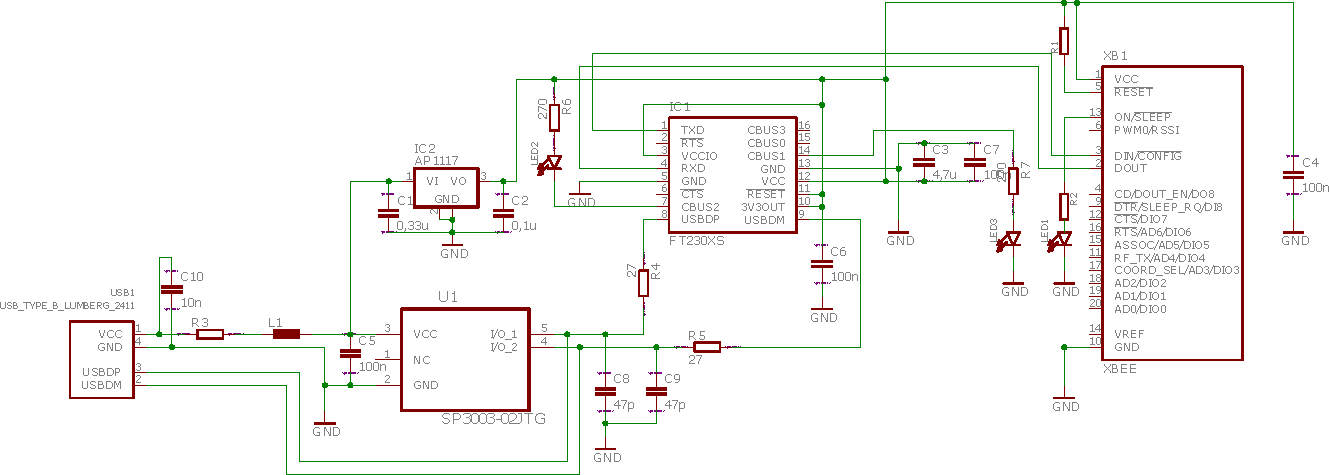
\includegraphics[width=1\textwidth]{schematic-xbee}
    \caption{Schema van de XBee USB module}
    \label{fig:schematic-xbee}
\end{figure}

\begin{figure}[h]
    \centering
    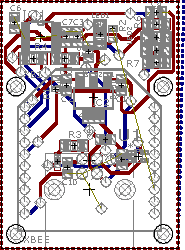
\includegraphics[width=0.5\textwidth]{board-xbee}
    \caption{Printplaat layout van de XBee USB module}
    \label{fig:board-xbee}
\end{figure}

\subsection{Controller board}
De hexapod bestaat uit 18 servomotoren die aangestuurd worden door een arbotiX robocontroller board (zie figuur \ref{fig:robocontroller-overview}). Deze controller bestaat uit een ATMega644P, een XBee module, servo connectoren en wat algemene in en outputs voor onderandere UART verbindingen.
\begin{figure}[h]
    \centering
    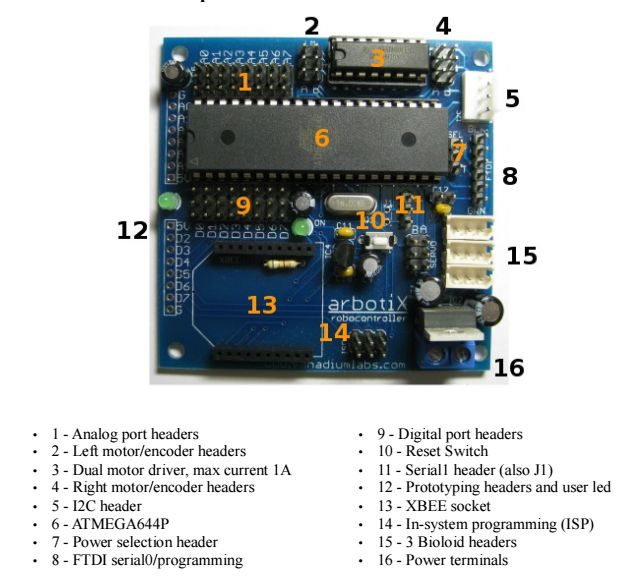
\includegraphics[width=0.8\textwidth]{robocontroller-overview.png}
    \caption{Robocontroller overzicht}
    \label{fig:robocontroller-overview}
\end{figure}


\newpage
\subsection{Software}
In dit hoofdstuk wordt de software van het project besproken. De software is onder te verdelen in diverse programma's met andere doeleinden.

\subsubsection{Lopen}
Wanneer de spin in de fysieke wereld moet lopen, en de koppeling tussen simulatie en de robot is gemaakt, moet het simulatie model ook een loop beweging uitvoeren. Hiervoor is een LUA programma geschreven, wat er voor zorgt dat het simulatiemodel zich voortbeweegt door de ruimte. Het programma wordt uitgevoerd binnen de simulatieomgeving zelf.

Het programma is geïnspireerd op het programma van de AntRobot, een standaard robot uit de V-REP bibliotheek. Deze robot komt qua fysieke kenmerken redelijk overeen met de hexapod. Dit model heeft ook een lichaam met daaraan zes poten welke op dezelfde wijze kunnen scharnieren als de hexapod. Dit maakt de beweging van de poten vrijwel identiek. Daarnaast maakt dit model eveneens gebruik van 'Inversed Kinematics', wat voor het toepassen van bepaalde aspecten van dit programma op de hexapod ideaal is.

Het ontwerp van de code is hetzelfde gebleven, alleen zijn er bepaalde aanpassingen gemaakt waardoor het toepasbaar is voor de hexapod. Het volledige programma is te vinden in de bijlage. 

Voor de testfase van het project is er voor gekozen om het model repeterende bewegingen te laten maken. In het huidige programma loopt de robot daarom ook een aantal seconden rechtdoor om vervolgens een bocht te maken naar rechts. Deze beweging wordt oneindig lang herhaald.


\subsubsection{Informatieverwerker}
Zoals in de opdracht staat omschreven, is het de bedoeling dat de fysieke robot aangestuurd kan worden door het simulatie model. Om dit te kunnen realiseren is er informatie nodig vanuit de simulatie. Het simulatiemodel is zo opgebouwd dat het overeenkomt met het fysieke model. Door deze overeenkomsten zouden de modellen het zelfde gedrag moeten vertonen bij gebruik van dezelfde parameters van de gewrichten.

De koppeling van simulatie naar de robot kan alleen worden gemaakt wanneer de simulatie in V-REP is gestart. In een Python programma wordt de verbinding gemaakt met de simulatieomgeving. Met behulp van de onderstaande regels code wordt deze verbinding tot stand gebracht. Het is eventueel ook mogelijk om het simuleren op een andere computer te doen dan de computer waarop het informatieverwerkende programma op draait(zie regel 190).

\lstinputlisting[language=Python, numberfirstline=true, firstnumber=189 , firstline=189, lastline=196, style=cstyle, caption=main.py - python informatieverwerker - Verbinding maken met de simulatieomgeving., label={connectvrep}]{./source-code/main.py}

Zodra het programma is gestart en de verbinding tussen de twee programma's tot stand is gebracht, worden de hoeken van de servomotoren uitgelezen. De hoeken worden ten opzichte van een bovenliggend object in de hirarchie van het model berekend. Om dit te verduidelijken is er als voorbeeld een afbeelding gemaakt van drie objecten die aan elkaar zijn verbonden.

\begin{figure}[h]
    \centering
    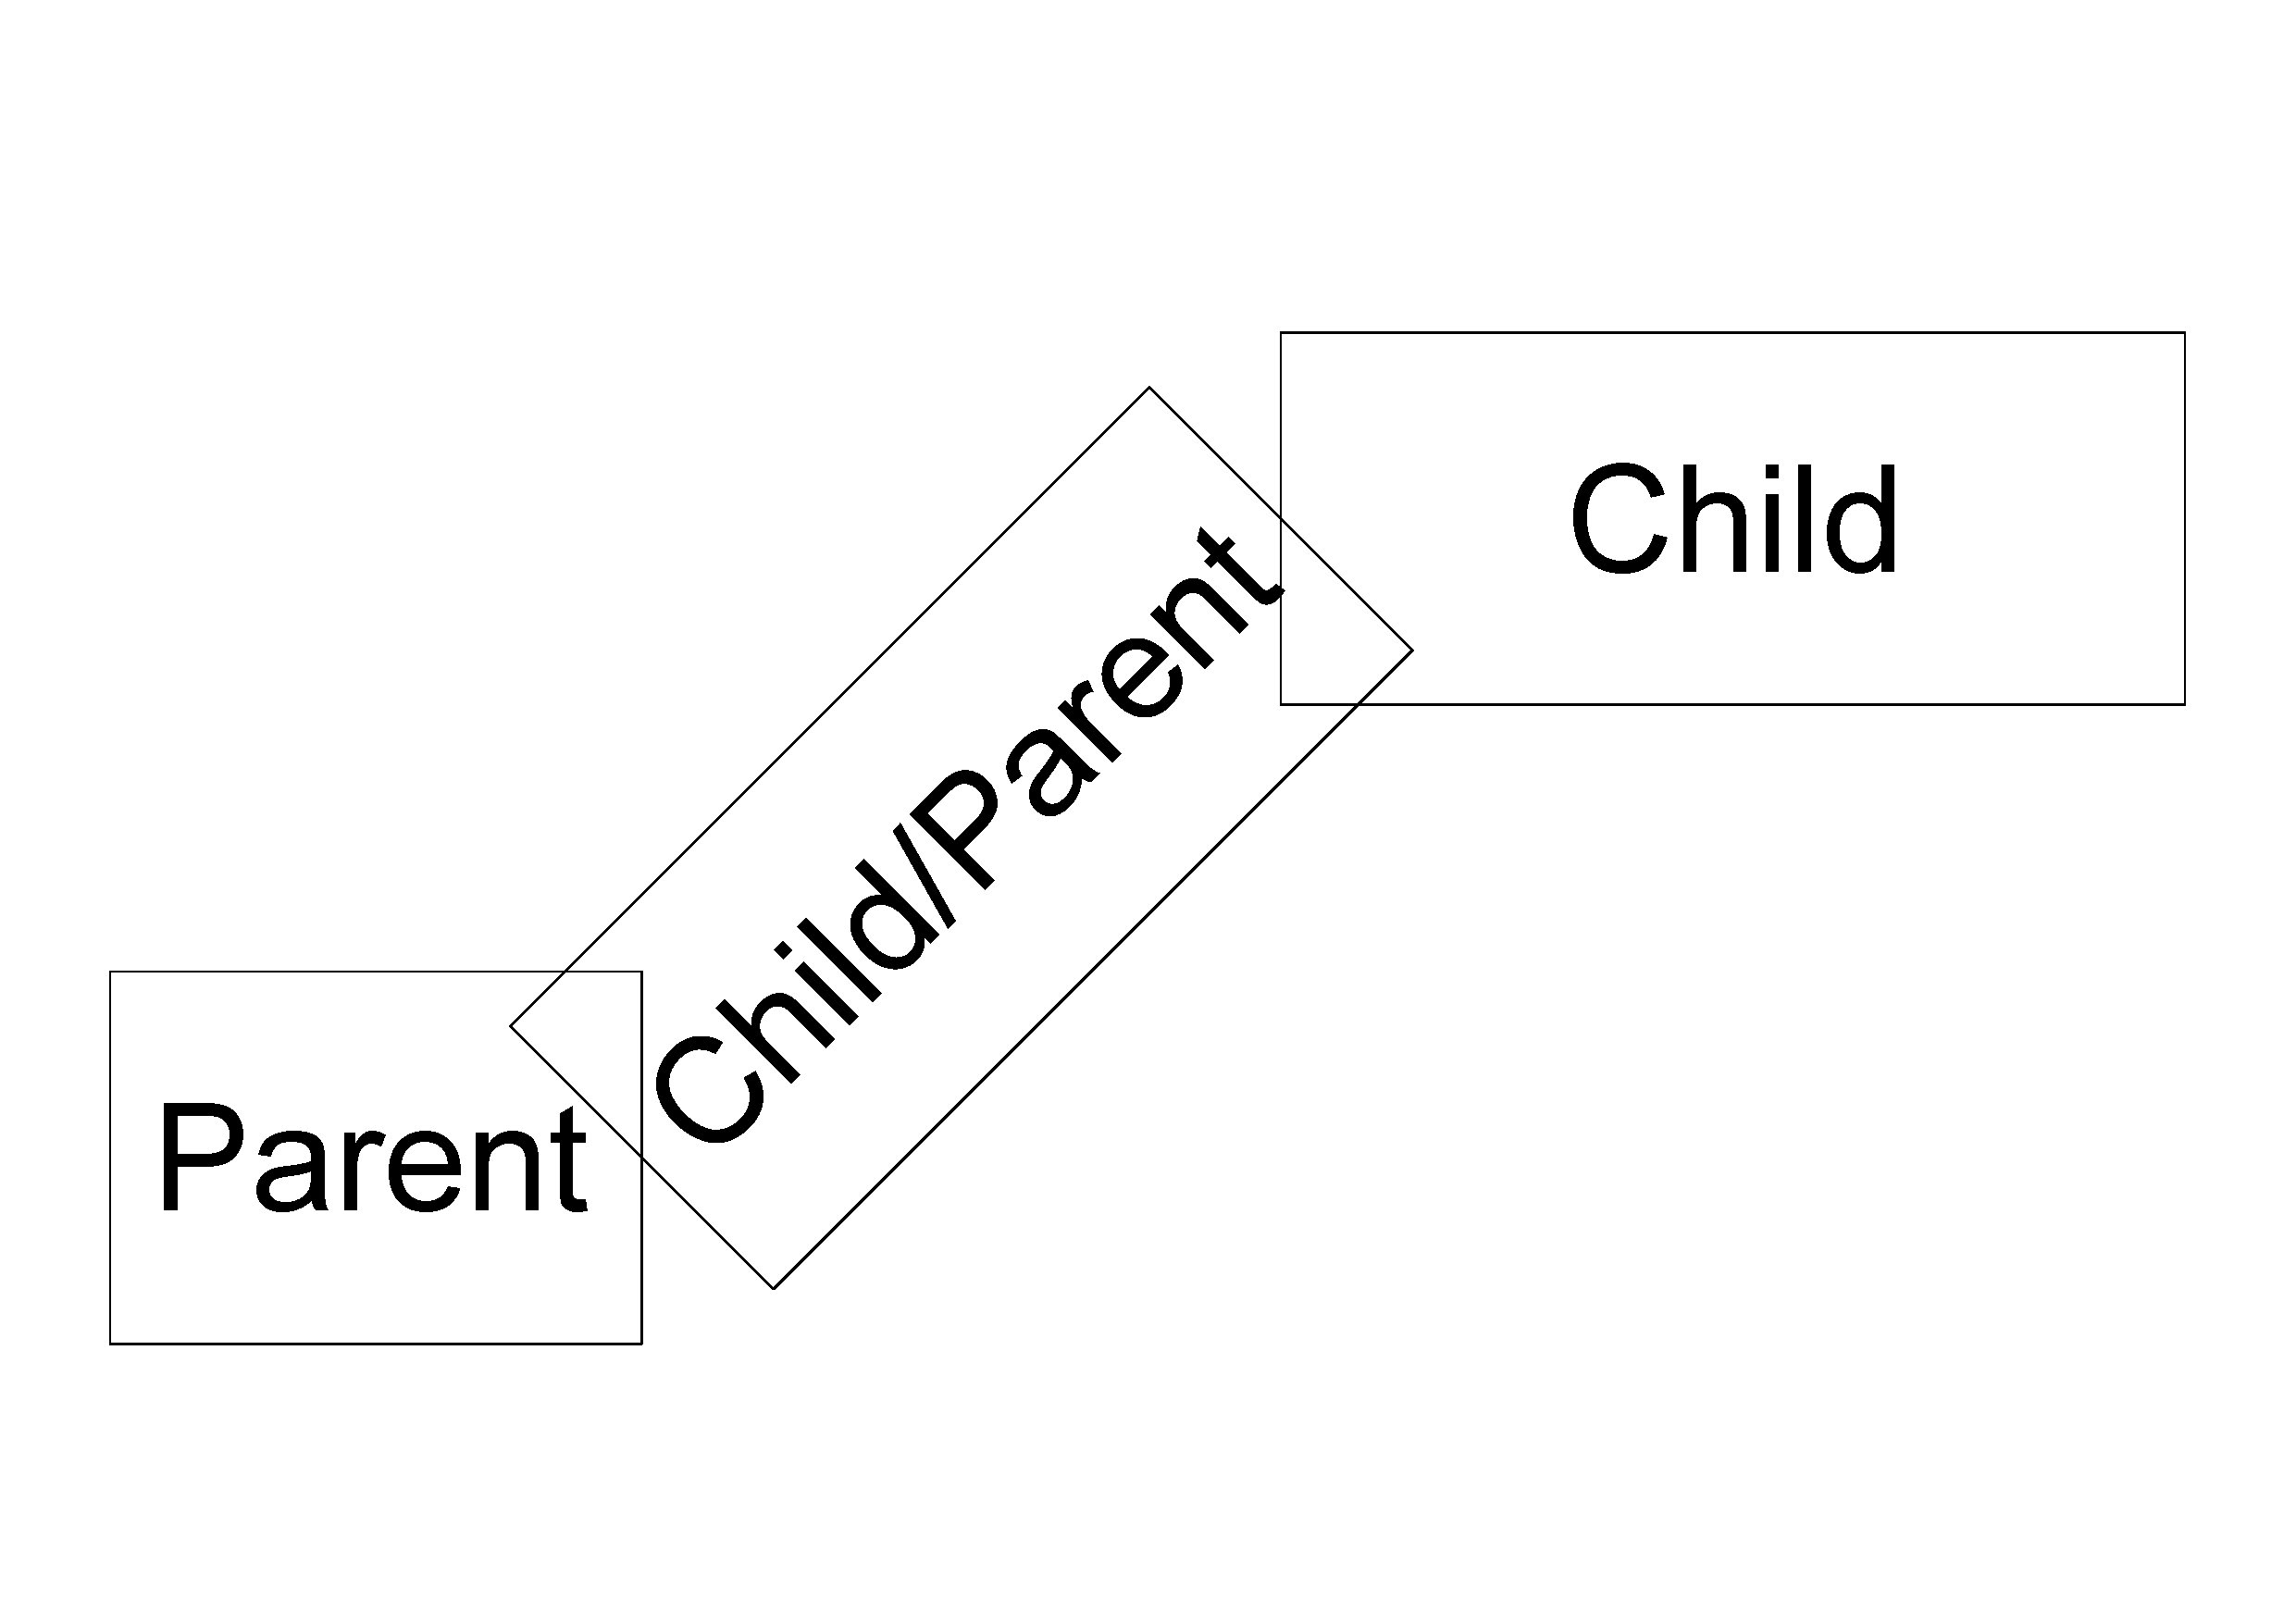
\includegraphics[width=1\textwidth]{hierarchi}
    \caption{Voorbeeld van een child/parent hierarchie van drie met elkaar verbonden objecten. De hoek tussen de parent en child is de hoek die nodig is in het programma.}
    \label{fig:hierarchi}
\end{figure}

De hoekverandering is dan in het geval van de hexapod altijd over \'e\'en van de drie dimensionale assen. Het uitlezen van de hoeken gebeurt met behulp van een programma wat per gewricht de hoek uitleest. Door gebruik te maken van de remote-API van V-REP is het extern aanroepen van functies mogelijk. De verkregen hoek wordt door de functie teruggegeven in radialen. In de onderstaande code wordt de hoek verkregen en omgerekend naar graden. Vervolgens wordt er nog een correctiefactor toegepast, omdat de toegepaste servomotoren op de hexapod 1023 stappen kunnen maken in plaats van 360.

\lstinputlisting[language=Python, numberfirstline=true, firstnumber=151 , firstline=151, lastline=156, style=cstyle, caption=main.py - python informatieverwerker - functie om de hoek tussen twee objecten op te vragen., label={getobjectangle}]{./source-code/main.py}

Naast de verbinding met het simulatieprogramma is er een externe draadloze verbinding nodig met de hexapod. Deze draadloze communicatie verloopt met behulp van het ZigBee protocol. Een zelf ontworpen printplaat met daarop een XBee module en een USB aansluiting moet worden aangesloten op de computer waarop het informatieverwerkende programma draait.

Het programma maakt verbinding met de COM poort van de computer waarop de printplaat met XBee module is aangesloten. Vervolgens wordt er met behulp van verschillende functies een verbinding tot stand gebracht. Zie hiervoor de volledige code die als bijlage is te vinden. 


\subsubsection{Aansturen servomotoren}
De servomotoren die gebruikt zijn de Dynamixel AX-18F. Deze motoren werken op 12 volt en kunnen maximaal 2,2 ampere aan stroom gebruiken.
Voor het aansturen gebruiken de motoren een eigen serieel protocol.\\\\
Het protocol werkt met een master die steeds een pakket over de communicatie bus stuurt en mogelijk een pakket terug kan krijgen. Elk pakket is gericht aan \'e\'en, meerdere of alle motoren (slaves).
De inhoud van een instructie pakket (master naar servo) bestaat uit de informatie uit tabel \ref{instructionpackage}.

\begin{table}[]
\centering
\caption{Instructie pakket van master naar servo.}
\label{instructionpackage}
\begin{tabular}{|l|l|l|l|l|l|l|l|}
\hline
0xFF & 0xFF & ID & Length & Instruction & Parameter0 & Parameters-n & Checksum \\ \hline
\end{tabular}
\end{table}

Twee maal '0xFF' geeft het begin van een pakket aan. Wanneer dit ontvangen wordt weet iedereen van de bus dat er een pakket aankomt.\\\\
Een 'ID' geeft het ontvangers ID aan. Elke servo heeft een uniek ID die gebruikt kan worden. Verder is er een speciaal BROADCAST id waar elke servo naar luistert.

\begin{figure}[h]
    \centering
    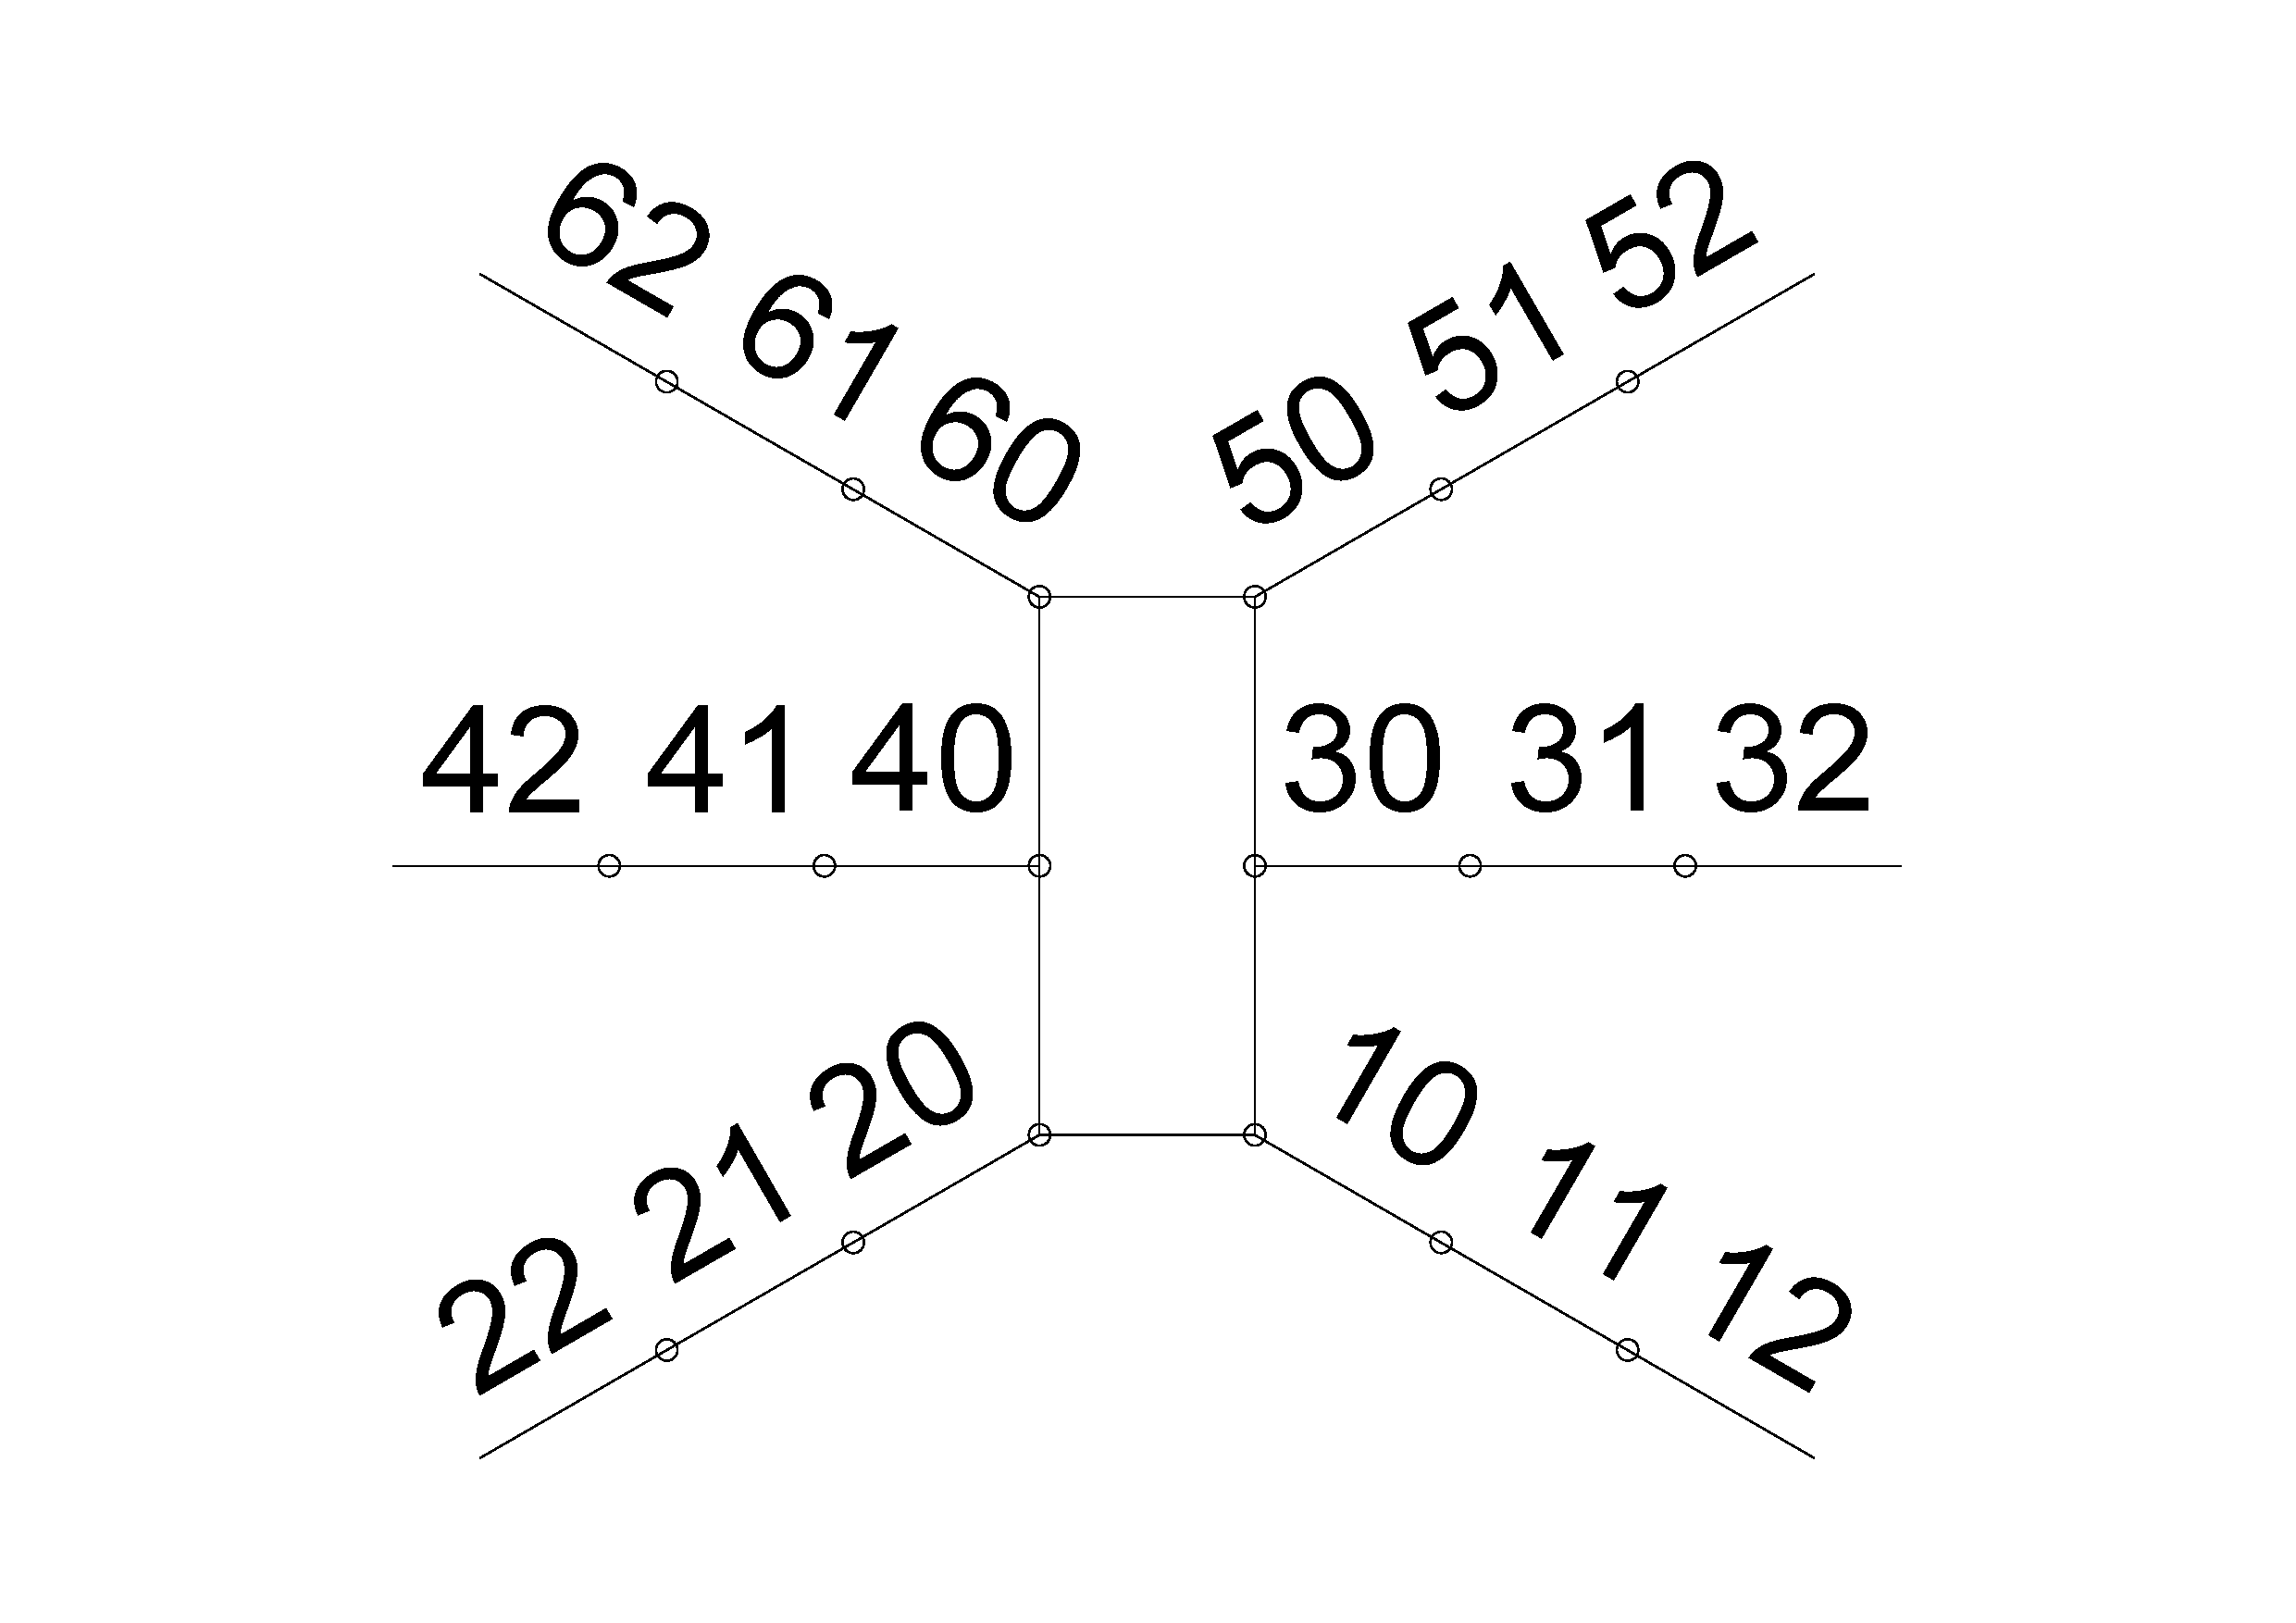
\includegraphics[width=0.8\textwidth]{hexapodid}
    \caption{Elke servomotor heeft een eigen ID, het nummer is bepaald aan de hand van de positie.}
    \label{fig:hexapodid}
\end{figure}



De parameter 'LENGTH' bevat de lengte van het pakket aan informatie. Hierdoor weet de ontvanger hoeveel parameters het kan verwachten\\\\
Een 'INSTRUCTION' is het type pakket. Dit kan een 'READ', 'WRITE' of 'SYNCWRITE' zijn. Bij READ word er een waarde uitgelezen, Bij WRITE een waarde weggeschreven en bij SYNCWRITE kan er bij meerdere servomotoren tegelijk worden geschreven.\\\\
De waarde 'PARAMETER0' is het lees/schrijf adres.
'PARAMETER-N' is alle informatie die weggeschreven moet worden. Bij een SYNCWRITE instructie bevat dit de servo ID's en DATA per servo zodat meerdere servo's tegelijk beschreven kunnen worden.\\\\
De 'CHECKSUM' bevat een checksum van het gehele pakket zodat gecontroleerd kan worden of alles goed is aangekomen.\\\\
Een 'status pakket' (servo naar master) bestaat uit de volgende stukken informatie:\\

\begin{table}[]
\centering
\caption{status pakket van servo naar master.}
\label{instructionpackage}
\begin{tabular}{|l|l|l|l|l|l|l|}
\hline
0xFF & 0xFF & ID & Length & Error & Parameters-n & Checksum \\ \hline
\end{tabular}
\end{table}

Net zoals bij een instructie pakket geeft tweemaal '0xFF' het begin van een pakket aan. Wanneer dit ontvangen wordt weet iedereen dat er een pakket aankomt.\\\\

De parameter 'ERROR' geeft een binaire code terug met de fouten die op dat moment actief zijn in de servo. Zo een fout kan bijvoorbeeld zijn: overbelasting, checksum fout of een ingangspanning fout.\\\\
PARAMETER-N geeft de informatie terug die door de instructie pakket is opgevraagd\\\\


\textbf{Implementatie}
Het controller board werkt met een ATMega644P waarbij de Servo connectoren direct aangesloten zijn op een UART ingang van de atmega. De servo communicatiebus werkt met een enkele seriele lijn en dat betekent dat zowel de verzend als de ontvang kant via dezelfde lijn werkt (half duplex). Daarom moet elke keer wanneer informatie verzonden wordt de ATMega UART ontvang hardware uitgezet worden. Andersom geldt dit ook, wanneer er informatie ontvangen wordt de ATMega UART verzend hardware uit worden gezet.\\
De AX18FWrite functie werkt vrij vanzelfsprekend. De UART Tx module wordt aangezet, de transmit buffer wordt leeg gehaald en vervolgens wordt de buffer weer gevuld met informatie van het pakketje. Op het eind wordt nog een checksum toegevoegd en de Tx module weer uitgezet.\\

\lstinputlisting[language=C, numberfirstline=true, firstnumber=46 , firstline=46, lastline=74, style=cstyle, caption=AX18ServoDriver.c - AX18Write functie, label={ax18write}]{./source-code/AX18ServoDriver.c}

De Read functie is iets uitgebreider omdat het de informatie echt moet kunnen analyseren. Eerst wordt een pakket verzonden naar de servo met een aanvraag voor informatie. Dit gebeurd op dezelfde manier zoals in de AX18FWrite functie. Daarna wacht de functie tot er informatie terug komt van de servo. Elke byte die dan terug komt wordt in een state machine gestopt die alles byte voor byte analyseert. Zo zijn state 1 en state 2 de start bytes. Wanneer een andere byte dan de start byte is gevonden wordt de state weer naar 0. De rest van de states zijn ook duidelijk.


\lstinputlisting[language=C, numberfirstline=true, firstnumber=119 , firstline=119, lastline=229, style=cstyle, caption=AX18ServoDriver.c - AX18Read functie, label={ax18write}]{./source-code/AX18ServoDriver.c}

\subsubsection{Communicatieprotocol}
Om de robot draadloos aan te sturen wordt er gebruik gemaakt van XBee modules. Deze modules werken via een seri\"e ele verbinding. XBee bevat de mogelijkheid om de seri\"e ele informatie in data pakketten te versturen om zo individuele pakketten te kunnen onderscheiden. Echter maken wij daar geen gebruik van om het geheel wat simpeler te houden. Dit betekent dat er \' e\'en continu\"e stroom van data is die geanalyseerd moet worden om losse informatieberichten te onderscheiden.\\
Dit wordt gedaan op dezelfde manier zoals de servo motoren worden aangestuurd. Het pakket begint wanneer er vier start bytes zijn gevonden. Daarna komt de lengte van de data, het commando, de data zelf en als laatst een checksum om het gehele pakket te controleren op fouten. Zie tabel \ref{transmit-xbee}. Deze pakketten kunnen op dit moment nog \'e\'en kant op worden gestuurd (van de computer naar de spin) maar dit is later gemakkelijk uit te breiden om ook de andere kant op te gaan op dezelfde manier zoals bij de servomotoren het geval is.
\begin{table}[h]
\centering
\begin{tabular}{lll}
\textbf{byte nr}      & \textbf{Example value}             & \textbf{meaning}                           \\
0-3          & 0x5A - 0x3C - 0x42 - 0x99 & Start bytes                       \\
4            & 0x02                      & Data length \\
5            & 0x00                      & Command                           \\
6-(6+length) & 0x60                      & Additional data                   \\
7+length     & 0xFF                      & Checksum (length, command and data)                  
\end{tabular}
\caption{XBee pakket}
\label{transmit-xbee}
\end{table}

\textbf{Implementatie}
Bij de implementatie van het communicatieprotocol is geprobeerd het systeem zo robuust mogelijk te maken. De communicatie over de XBee werkt als een seriele lijn waar een lange stroom aan informatie uitkomt. Omdat de XBee ook met buffers werkt en bij draadloos verkeer alle bytes niet altijd aankomen en opnieuw verzonden moeten worden kan het voorkomen dat er 1 byte binnenkomt en soms 25 bytes. Elke byte moet verwerkt worden en bytes die een tijd later aankomen kunnen nog horen bij een pakket die eerder is begonnen.\\
Om dit allemaal in goede banen te leiden is er een  'XBee\_ communication\_ processSerialData' functie gemaakt waar de staat van een pakket wordt opgeslagen en het pakket via meerdere stukken opgebouwd kan worden. Deze functie werkt ook met een state machine, het grote verschil is dat het pakket inclusief de ontvang staat globaal opgeslagen wordt. Verder kunnen pakketten worden opgeslagen en direct door worden gegaan met het analyseren van de rest van de informatie. De pakketten worden opgeslagen in een ringbuffer hierdoor kan de buffer nooit overstromen met te veel informatie maar zullen de meest oude pakketten verwijderd worden van de buffer zodat de nieuwste pakketten in ieder geval nog uitgelezen kunnen worden.\\
\lstinputlisting[language=C, numberfirstline=true, firstnumber=119 , firstline=77, lastline=146, style=cstyle, caption=XbeeCom.c - processSerialData functie, label={processSerialData}]{./source-code/XbeeCom.c}
\newpage


\section{Discussie en resultaten}
In de specificatie van dit raamwerk staan noodzakelijke en gewenste specificaties.
Het primaire doel van het project was een verbinding cre\"eren tussen de fysieke hexapod en het simulatiemodel. Deze verbinding moest draadloos zijn om de hexapod niet te beperken in zijn bewegingsvrijheid. Het doel van deze verbinding was dat het simulatiemodel de fysieke robot kon aansturen. Vanwege deze reden was het van belang dat de maatgeving van de de modellen overeen kwamen met elkaar. Om te voorkomen dat de robot zichzelf zou beschadigen was het van belang dat het simulatiemodel geen onmogelijke commando's naar de fysieke robot zou sturen.

Alle bovengenoemde noodzakelijke specificaties zijn behaald. De hexapod kan draadloos aangestuurd worden vanuit het simulatiemodel en verricht exact de zelfde handeling. Het simulatiemodel is zo ingesteld dat het onmogelijk is gemaakt dat de robot zichzelf kan beschadigen door een verkeerde stuuractie. Daarnaast vinden er op verschillende plaatsen in de software checksums plaats die corrupte berichten filteren uit de informatieoverdracht.

De gewenste specificaties zijn door verschillende redenen niet gerealiseerd. Dat heeft te maken met 

\newpage
\section{Aanbevelingen}
In het voorgaande hoofdstuk bleek dat niet alle gewenste specificaties zijn behaald. Dit blijven opties om te implementeren in de toekomst. 

Het huidige model heeft nog een aantal beperkingen. Zo is het momenteel niet mogelijk om bijvoorbeeld de poot van de fysieke hexapod te bewegen en dit terug te zien in het simulatiemodel. Die communicatie verloopt nu namelijk e\"e\"n richting op. 

Daarnaast kwam het team er achter dat de huidige hardware (de robocontroller) toch nog een aantal beperkingen heeft. Zo bleek de ATMega moeite te hebben met het verwerken van de draadloze informatieoverdracht. Dit resulteerde in het falen van checksum en het traag reageren van de fysieke robot. Momenteel word iedere 20 milliseconde een update van de stand van de poten opgevraagd om een nog enig sinds vloeiende beweging te cre\"eeren. Achteraf gezien was het wellicht toch beter om een eigen "robocontroller' te ontwikkelen.


\newpage


\section{Bijlage}

\newpage

\section{Bibliografie}
\bibliography{references}
\bibliographystyle{IEEEtran}


\end{document}